\subsection{Descrizione dello Scopo}
Lo scopo principale dell'applicativo \textbf{PishTrap} è fornire un sistema semplice ed efficace per il rilevamento di attacchi di phishing attraverso l'analisi automatica delle email. 

L'applicativo permette di:

\begin{itemize}
    \item Identificare URL e contenuti sospetti utilizzando API esterne e dati locali.
    \item Raggruppare email di phishing in categorie per migliorare la comprensione delle minacce.
\end{itemize}

Questo approccio non solo aumenta la sicurezza dell'utente, ma contribuisce anche alla sua formazione nella prevenzione di attacchi futuri.

\subsection{Requisiti e Casi d'Uso}
I requisiti funzionali dell'applicativo saranno documentati utilizzando una \textbf{matrice di tracciabilità dei requisiti}. Questa matrice consente di tracciare i requisiti rispetto ai casi d'uso correlati e alla loro priorità, fornendo una visione chiara delle funzionalità implementate.

\begin{table}[h!]
\centering
\begin{tabular}{|c|l|c|l|}
\hline
\textbf{ID Requisito} & \textbf{Descrizione}           & \textbf{Priorità} & \textbf{Casi d'Uso Collegati} \\ \hline
CD-1                 & Login dell'utente nell'applicazione    & Alta              & CD-2                \\ \hline
CD-2                 & Logout    & Alta             & CD-1                 \\ \hline
CD-3                 & Autenticazione con account Google    & Alta            & CD-1   \\ \hline
CD-4                 & Scansione email non lette    & Alta             & CD-1                 \\ \hline
CD-5                 & Scansione email per giorno    & Media             & CD-1                 \\ \hline
\end{tabular}
\caption{Matrice di tracciabilità dei requisiti funzionali}
\label{tab:tracciabilita-requisiti}
\end{table}

\noindent
Ogni requisito è identificato da un codice univoco (\textbf{ID Requisito}), classificato per priorità (\textbf{Alta}, \textbf{Media}, \textbf{Bassa}) e collegato ai casi d'uso che lo soddisfano.

La matrice sarà aggiornata iterativamente durante lo sviluppo per garantire che tutti i requisiti funzionali siano tracciati e implementati correttamente.

Oltre ai requisiti funzionali, l'applicativo \textbf{PishTrap} deve rispettare una serie di requisiti non funzionali per garantire prestazioni, sicurezza e affidabilità. Di seguito sono riportati i principali requisiti non funzionali:

\begin{itemize}
    \item \textbf{Prestazioni}: L'applicativo deve garantire una risposta rapida durante l'interazione dell'utente, specialmente per operazioni critiche come il login e la scansione delle email.
    \item \textbf{Scalabilità}: Il sistema deve essere in grado di gestire un aumento del numero di utenti senza degradare significativamente le prestazioni.
    \item \textbf{Sicurezza}: Tutti i dati sensibili devono essere protetti tramite comunicazioni cifrate e conformità alle normative sulla privacy.
    \item \textbf{Affidabilità}: Il sistema deve essere stabile e garantire la disponibilità continua dei servizi principali, riducendo al minimo i tempi di inattività.
    \item \textbf{Usabilità}: L'applicativo deve essere intuitivo e facile da usare, con un'interfaccia chiara che permetta agli utenti di completare le operazioni senza difficoltà.
    \item \textbf{Manutenibilità}: Il codice e l'architettura del sistema devono essere progettati in modo da agevolare future modifiche e aggiornamenti.
    \item \textbf{Compatibilità}: L'applicazione deve essere compatibile con dispositivi Android che supportano versioni moderne del sistema operativo e garantire un funzionamento ottimale.
    \item \textbf{Conformità}: Il sistema deve rispettare le normative sulla protezione dei dati personali, come il GDPR, e fornire una chiara informativa sulla privacy agli utenti.
\end{itemize}

\noindent
Questi requisiti saranno monitorati e verificati durante tutte le fasi di sviluppo, attraverso test specifici e simulazioni, per assicurare il rispetto degli standard di qualità definiti.

\subsection{Diagramma dei Casi d'Uso}
Il diagramma dei casi d'uso rappresentato nella Figura~\ref{fig:usecase} illustra le principali funzionalità offerte dall'applicativo \textbf{PishTrap} e le interazioni tra l'utente e il sistema.

\begin{figure}[h!]
\centering
\includegraphics[width=0.8\textwidth]{diagrammiUML/Use case.pdf}
\caption{Diagramma dei Casi d'Uso}
\label{fig:usecase}
\end{figure}

\subsection{Diagramma di Deployment}
Il \textbf{Diagramma di Deployment} riportato nella Figura~\ref{fig:deployment} illustra l'architettura di distribuzione dell'applicativo \textbf{PishTrap}, mostrando come i diversi componenti del sistema sono distribuiti tra i dispositivi hardware e i nodi software.

Il diagramma evidenzia:
\begin{itemize}
    \item Il dispositivo utente (Smartphone Android) con l'applicazione Flutter.
    \item Il WebServer AWS, che ospita il back-end e i suoi servizi modulari.
    \item Le connessioni con servizi esterni come Google Cloud (OAuth 2.0, Gmail API, Safe Browsing API) e PhishTank.
    \item La comunicazione con il database MongoDB Atlas per l'archiviazione dei dati.
\end{itemize}

\noindent
Questo diagramma riflette diversi stili architetturali che caratterizzano il sistema:
\begin{itemize}
    \item \textbf{MVC (Model-View-Controller)}: È chiaramente visibile nella separazione tra il front-end (View), il back-end (Controller) e il database (Model).
    \item \textbf{Three-Tier Architecture}: Mostra la stratificazione in tre livelli principali: Presentazione (Flutter), Logica (back-end su AWS) e Persistenza dei dati (MongoDB).
    \item \textbf{Client-Server}: Il modello base di comunicazione tra il client (app Flutter) e il server back-end.
    \item \textbf{Microservizi}: Alcuni componenti del back-end, come il modulo per l'autenticazione OAuth 2.0 o l'integrazione con API esterne, possono essere visti come microservizi che operano indipendentemente.
\end{itemize}

\begin{figure}[h!]
\centering
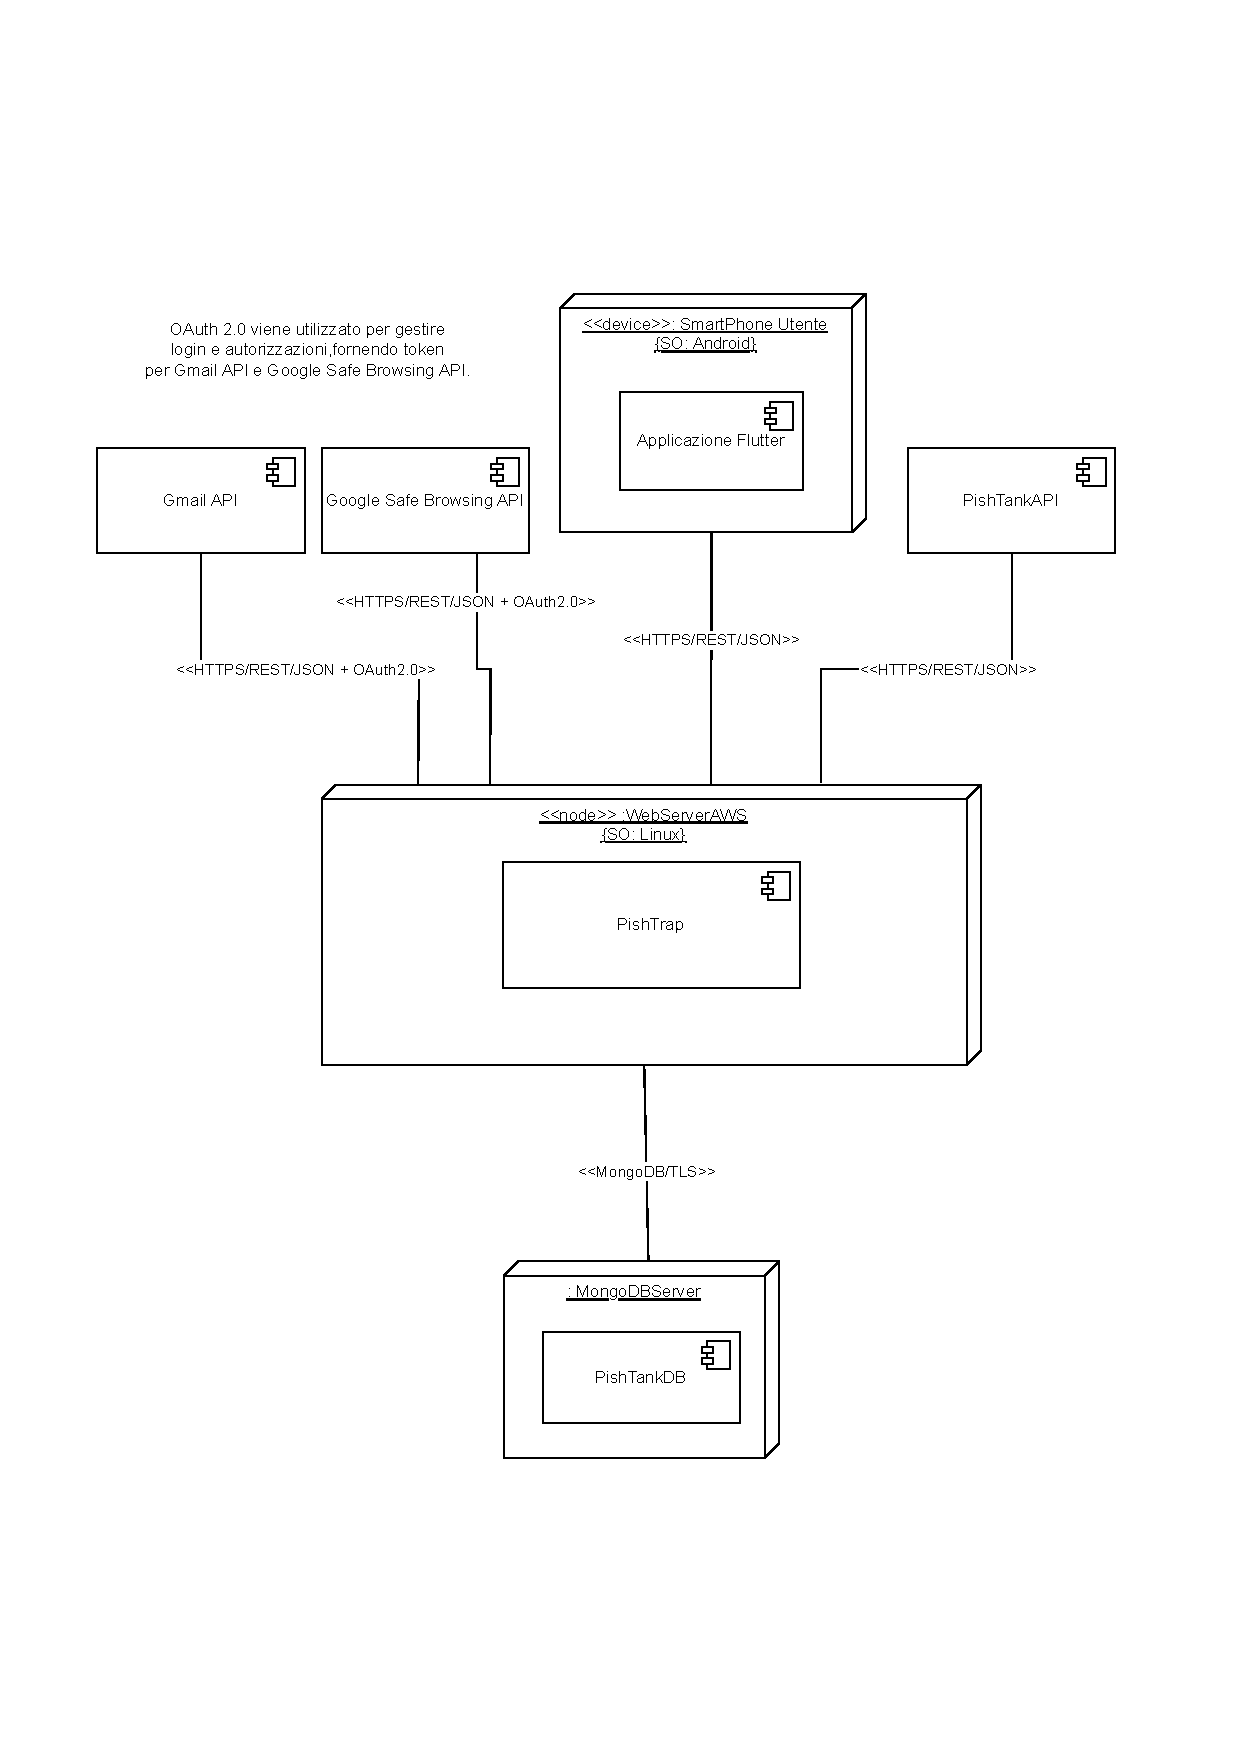
\includegraphics[width=0.8\textwidth]{diagrammiUML/Deployment.pdf}
\caption{Diagramma di Deployment}
\label{fig:deployment}
\end{figure}

\subsection{Toolchain Utilizzata}
Per lo sviluppo e il deployment dell'applicativo \textbf{PishTrap}, è stata utilizzata una toolchain composta da tecnologie e strumenti moderni che garantiscono efficienza, scalabilità e flessibilità. Di seguito è riportata una lista completa degli strumenti utilizzati, con una breve descrizione delle loro funzionalità principali:

\begin{itemize}
    \item \textbf{Flutter}: Framework open-source sviluppato da Google per creare applicazioni mobili, web e desktop con un'unica codebase. Utilizzato per lo sviluppo dell'interfaccia utente dell'applicativo su dispositivi Android.
    \item \textbf{GitHub}: Piattaforma per il versionamento del codice e la collaborazione tra sviluppatori. Utilizzato per il controllo delle versioni del progetto, la gestione dei branch delle iterazioni e la documentazione del codice.
    \item \textbf{PhishTank API}: Servizio online che fornisce un database costantemente aggiornato di URL noti per il phishing. Utilizzato per verificare l'affidabilità degli URL presenti nelle email.
    \item \textbf{MongoDB}: Database NoSQL cloud-based utilizzato per l'archiviazione dei dati analizzati, come email sospette e risultati delle scansioni.
    \item \textbf{AWS (Amazon Web Services)}: Piattaforma cloud utilizzata per il deployment del back-end, con particolare utilizzo di servizi come EC2 per l'esecuzione dei servizi server-side.
    \item \textbf{Python}: Linguaggio di programmazione utilizzato per implementare la logica del back-end, come l'integrazione con API esterne, la gestione dei dati e l'elaborazione degli algoritmi di clustering (K-means).
    \item \textbf{Google Cloud (Gmail API e Google Safe Browsing API)}: Servizi di Google Cloud utilizzati per l'integrazione con account Gmail (accesso e lettura delle email) e per il controllo della sicurezza degli URL tramite Google Safe Browsing.
    \item \textbf{Postman}: Strumento per testare e documentare le API REST. Utilizzato per verificare la correttezza delle API implementate nel back-end e per simulare le richieste provenienti dal client.
    \item \textbf{Draw.io}: Strumento per la creazione di diagrammi UML e schemi architetturali. Utilizzato per rappresentare graficamente i diagrammi di componenti, deployment e casi d'uso.
    \item \textbf{Overleaf}: Piattaforma online per l'editing collaborativo di documenti in LaTeX. Utilizzata per creare e gestire la documentazione del progetto, inclusi report e diagrammi integrati.
\end{itemize}

\noindent
Questa toolchain è stata scelta per garantire uno sviluppo rapido ed efficace, assicurando al contempo la scalabilità, e una documentazione chiara e ben strutturata.
